\documentclass[compress]{beamer}
\usepackage{ifthen}
\usepackage{verbatim}
\usepackage[procnames]{listings}
\usepackage{array}

\xdefinecolor{lightyellow}{rgb}{1.,1.,0.25}
\xdefinecolor{darkblue}{rgb}{0.1,0.1,0.7}

\setbeamertemplate{navigation symbols}{}
\setbeamertemplate{headline}{\mbox{ } \hfill
\begin{minipage}{5.5 cm}
\vspace{-0.75 cm} \small
\end{minipage} \hfill
\begin{minipage}{4.5 cm}
\vspace{-0.75 cm} \small
\begin{flushright}
\ifthenelse{\equal{\insertpagenumber}{1}}{}{Jim Pivarski \hspace{0.2 cm} \insertpagenumber/\pageref{numpages}}
\end{flushright}
\end{minipage}\mbox{\hspace{0.2 cm}} \hspace{0.01 cm} \vspace{-1.05 cm}}

\newcommand{\s}[1]{{\mbox{\scriptsize #1}}}

\definecolor{gray}{gray}{0.5}
\definecolor{green}{rgb}{0,0.5,0}
\definecolor{brown}{rgb}{0.5,0.25,0}
\definecolor{lightgreen}{rgb}{0,0.7,0}
\definecolor{darkgreen}{rgb}{0,0.4,0}
\definecolor{purple}{rgb}{0.5,0,0.5}
\definecolor{darkred}{rgb}{0.5,0,0}
\lstset{
language=python,
basicstyle=\ttfamily\scriptsize,
moredelim=**[is][\color{black}]{$}{$},
moredelim=**[is][\color{black}]{>}{>}
}

% \lstset{
% language=python,
% basicstyle=\ttfamily\scriptsize,
% stringstyle=\color{brown},
% showstringspaces=false,
% alsoletter={1234567890},
% otherkeywords={\ , \}, \{},
% keywordstyle=\color{blue},
% emph={access,and,as,break,class,continue,def,del,elif,else,%
% except,exec,finally,for,from,global,if,import,in,is,%
% lambda,not,or,pass,print,raise,return,try,while,assert,yield},
% emphstyle=\color{darkgreen}\bfseries,
% emph={[2]self,other},
% emphstyle=[2]\color{darkgray},
% emph={[4]ArithmeticError,AssertionError,AttributeError,BaseException,%
% DeprecationWarning,EOFError,Ellipsis,EnvironmentError,Exception,%
% False,FloatingPointError,FutureWarning,GeneratorExit,IOError,%
% ImportError,ImportWarning,IndentationError,IndexError,KeyError,%
% KeyboardInterrupt,LookupError,MemoryError,NameError,None,%
% NotImplemented,NotImplementedError,OSError,OverflowError,%
% PendingDeprecationWarning,ReferenceError,RuntimeError,RuntimeWarning,%
% StandardError,StopIteration,SyntaxError,SyntaxWarning,SystemError,%
% SystemExit,TabError,True,TypeError,UnboundLocalError,UnicodeDecodeError,%
% UnicodeEncodeError,UnicodeError,UnicodeTranslateError,UnicodeWarning,%
% UserWarning,ValueError,Warning,ZeroDivisionError,abs,all,any,apply,%
% basestring,bool,buffer,callable,chr,classmethod,cmp,coerce,compile,%
% complex,copyright,credits,delattr,dict,dir,divmod,enumerate,eval,%
% execfile,exit,file,filter,float,frozenset,getattr,globals,hasattr,%
% hash,help,hex,id,input,int,intern,isinstance,issubclass,iter,len,%
% license,list,locals,long,max,min,object,oct,open,ord,pow,property,%
% quit,raw_input,reduce,reload,repr,reversed,round,set,setattr,%
% slice,sorted,staticmethod,str,sum,super,tuple,type,unichr,unicode,%
% vars,xrange,zip},
% emphstyle=[4]\color{purple}\bfseries,
% upquote=true,
% morecomment=[s][\color{lightgreen}]{"""}{"""},
% commentstyle=\color{red}\slshape,
% literate={>>>}{\textbf{\textcolor{darkred}{>{>}>}}}3%
%          {...}{{\textcolor{gray}{...}}}3,
% procnamekeys={def,class},
% procnamestyle=\color{blue}\textbf,
% framexleftmargin=1mm, framextopmargin=1mm,
% rulesepcolor=\color{blue},#1,
% moredelim=**[is][\color{purple}]{$}{$},
% moredelim=**[is][\color{blue}]{>}{>}
% }

\begin{document}
\begin{frame}
\vfill
\begin{center}
\textcolor{darkblue}{\Large Physics and Data Science: \\\vspace{0.2 cm} Reflections from a physicist in industry}

\vfill
\begin{columns}
\column{0.3\linewidth}
\begin{center}
\large
Jim Pivarski
\end{center}
\end{columns}

%% \begin{columns}
%% \column{0.3\linewidth}
%% \begin{center}
%% \scriptsize
%% {\it Fermilab}
%% \end{center}
%% \end{columns}

\vfill
October 30, 2015

\end{center}
\end{frame}

\small

\begin{frame}
\frametitle{My trajectory}
\begin{description}
\item[1999--2006:] Graduate work on CLEO, a medium-sized collaboration, Ph.D.\ from Cornell.
\item[2006--2011:] Postgraduate work on CMS, a large collaboration, with Texas A\&M University.
\begin{itemize}\setlength{\itemsep}{0.2 cm}
\item Commissioning, mostly muon detector alignment.
\item Search for leptonic jets in early LHC data.
\end{itemize}
\item[2011--now:] Data scientist for Open Data Group, a small consulting firm with clients in large companies.
\begin{itemize}\setlength{\itemsep}{0.2 cm}
\item Analyzed data from hyperspectral satellite photos, automobile traffic, network traffic, web trends, Twitter sentiment, geolocation, Chicago crime, etc.
\item Implemented data mining models with variations.
\item Created the Portable Format for Analytics (PFA), a data mining model interchange format in JSON.
\end{itemize}
\end{description}
\end{frame}

\begin{frame}
\frametitle{My trajectory}

PFA has been my largest project: a successor to PMML (Predictive Model Markup Language), PFA simplifies the representation of statistical models and adds basic control constructs. Basically, a programming language in JSON with a large library of data mining primitives.

\vspace{0.2 cm}
\mbox{ } \hfill 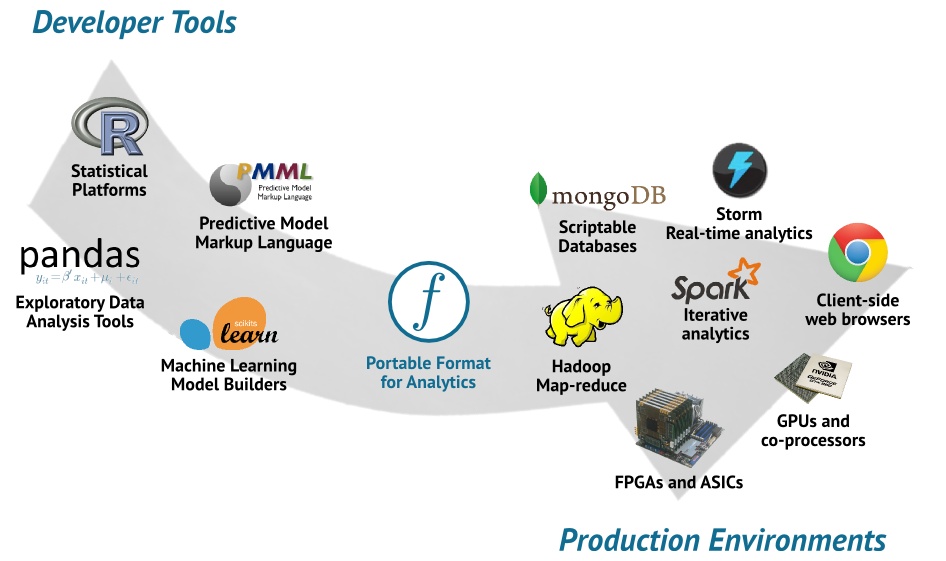
\includegraphics[width=0.7\linewidth]{PLOTS/pfatoeverything.png} \hfill \mbox{ }

\vspace{0.2 cm}
Recently adopted by the Data Mining Group (DMG), the organization that standardized and maintains PMML.

\vspace{0.2 cm}
\mbox{ } \hfill {\tt \textcolor{blue}{http://dmg.org}} \hfill \mbox{ }

\end{frame}

\begin{frame}
\frametitle{My trajectory}
\begin{center}
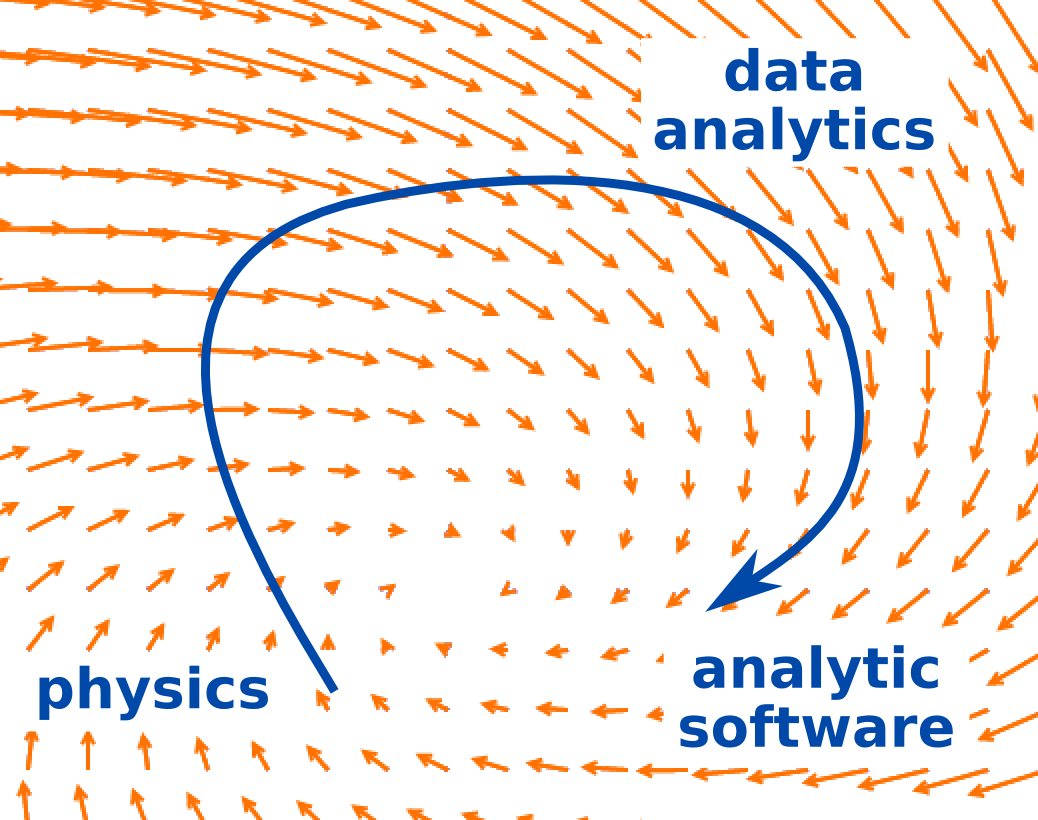
\includegraphics[width=0.8\linewidth]{PLOTS/vectorfield2_annotated.png}
\end{center}
\end{frame}

\begin{frame}
\frametitle{Outline}
\begin{itemize}\setlength{\itemsep}{0.75 cm}
\item What is data science?
\item Statistical techniques that aren't often used in HEP
\item Software tools: Hadoop, Spark, and all that
\item Trends in analytic programming
\end{itemize}
%% \hspace{-0.83 cm} \textcolor{darkblue}{\Large Outline2}
\end{frame}

\section*{What is data science?}
\begin{frame}
\begin{center}
\Huge \textcolor{blue}{What is data science?}
\end{center}
\end{frame}

\begin{frame}
\frametitle{What is data science?}
\vspace{0.5 cm}
Embarrassingly, most answers to this question come from Twitter\ldots
\begin{itemize}
\item ``A data scientist is a statistician who lives in San Francisco.''
\item ``A data scientist is better at statistics than a software engineer and better at programming than a statistician.''
\item ``A data scientist is a business analyst with a Mac.''
\end{itemize}

\vspace{0.2 cm}
\begin{center}
\uncover<2->{\fbox{\begin{minipage}{0.9\linewidth}
Data science is the application of statistical techniques to business decisions with an emphasis on software development and large-scale deployment (a.k.a.~``big data'').
\end{minipage}}}

\vspace{0.5 cm}
\uncover<3->{\fbox{\begin{minipage}{0.9\linewidth}
In other words, what high-energy physicists do, but applied to business decisions.
\end{minipage}}}
\end{center}
\end{frame}

\begin{frame}
\frametitle{What is data science?}
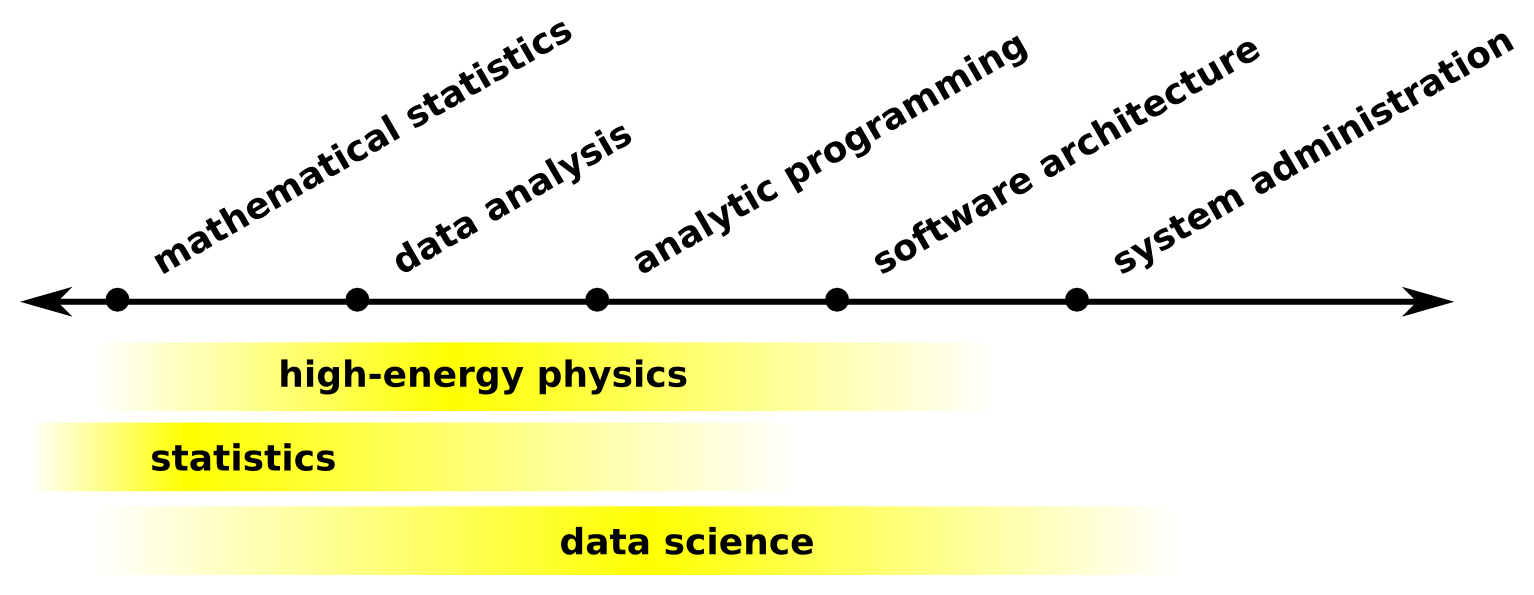
\includegraphics[width=\linewidth]{PLOTS/spectrum_of_data_science.png}

\vfill
\uncover<2>{Because of the overlap, many data scientists come from physics, but knowledge can flow the other way, too.}
\end{frame}

\section*{Statistical techniques}
\begin{frame}
\begin{center}
\Huge \textcolor{blue}{Statistical techniques}
\end{center}
\end{frame}

\begin{frame}
\frametitle{Fundamentals: what is a model?}
\vspace{0.2 cm}
\only<1>{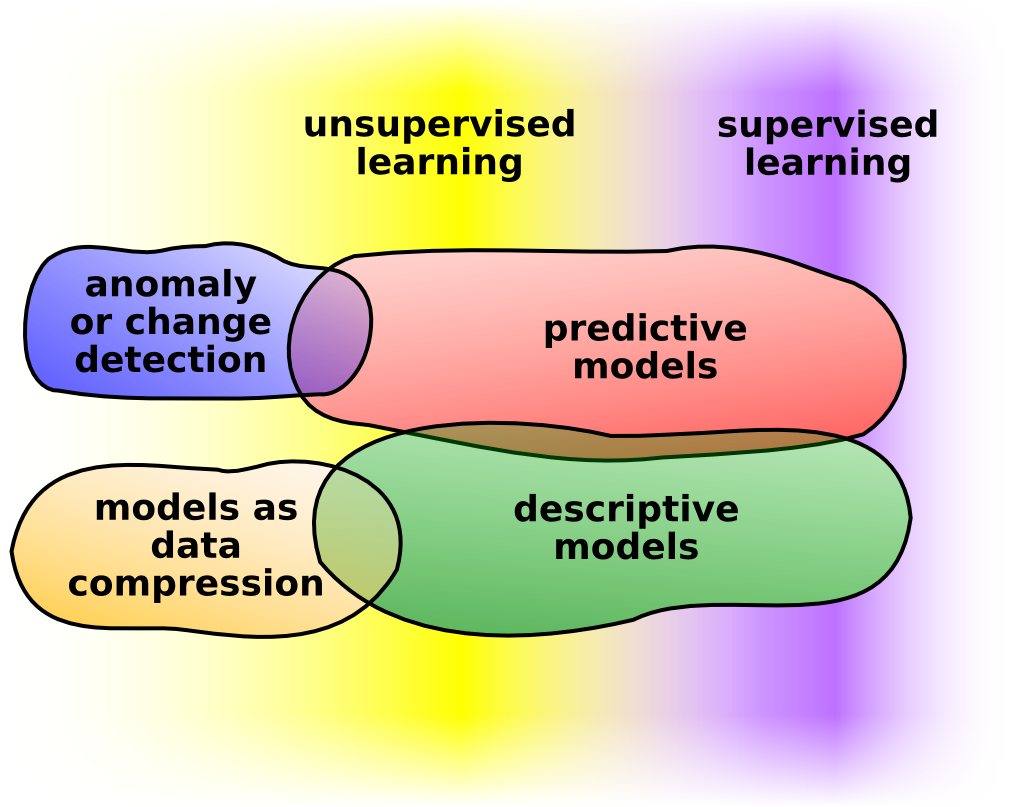
\includegraphics[width=\linewidth]{PLOTS/types_of_models.png}}
\only<2>{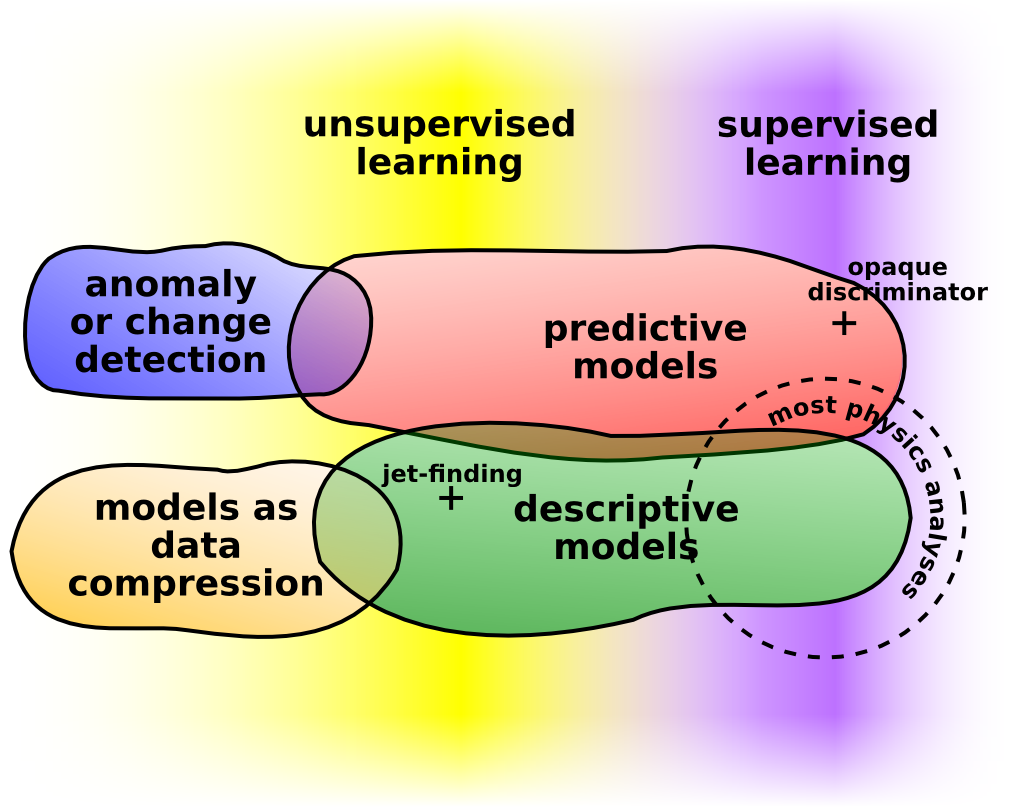
\includegraphics[width=\linewidth]{PLOTS/types_of_models_2.png}}
\end{frame}

\begin{frame}
\frametitle{Fundamentals: what is a model?}
\begin{description}
\item<1->[Descriptive:] Model is the final product, revealing an underlying relationship in the data: e.g.\ the Standard Model.
\item<1->[Predictive:] Model is a means to performing predictions and is judged on the quality of those predictions: e.g.\ stock predictions.
\item<2->[Supervised:] Training procedure accentuates differences between two labeled datasets: e.g.\ signal and background Monte Carlo.
\item<2->[Unsupervised:] Training procedure finds patterns on its own: e.g.\ groups of nearby particles are a jet.
\item<3->[Anomaly detection:] Model describes the normal situation to identify unusual cases or changes: e.g.\ data quality monitor.
\item<3->[Data compression:] Model summarizes data for the sake of describing it with fewer bits: e.g.\ image compression.
\end{description}
\end{frame}

\begin{frame}
\frametitle{Potential applications in physics}

\begin{columns}
\column{0.5\linewidth}
Some quantities, such as the LHC beamspot, are stable for long periods of time but might jump at discrete times.

\vspace{0.2 cm}
Want to identify jumps and combine statistics in the stable periods.
\column{0.5\linewidth}
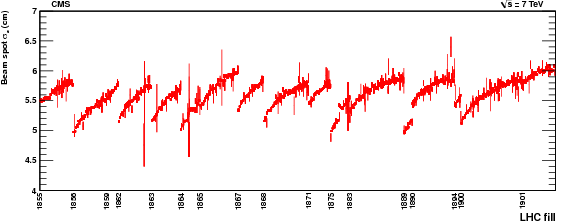
\includegraphics[width=\linewidth]{PLOTS/figs_2011_beamSpotAndPV_BeamSpot_Selected2011_sigmaZ.png}
\end{columns}

\only<2->{\vspace{0.2 cm}
\begin{itemize}
\only<2>{\item Generalized Likelihood Ratio (GLR) is a change detection technique that finds the time when one distribution jumps to another using a maximum likelihood scan.}
\only<3>{\item Regression trees can \\ use time as a regressor \\ to partition the \\ sequence into periods \\ of minimal variance \\ (or minimal linear-fit \\ $\chi^2$, etc.).}
\only<4>{\item Hierarchical clustering, especially single-linkage, groups chains of gradually changing parameters and splits at the biggest jumps.}
\end{itemize}}

\only<2>{\mbox{ } \hfill 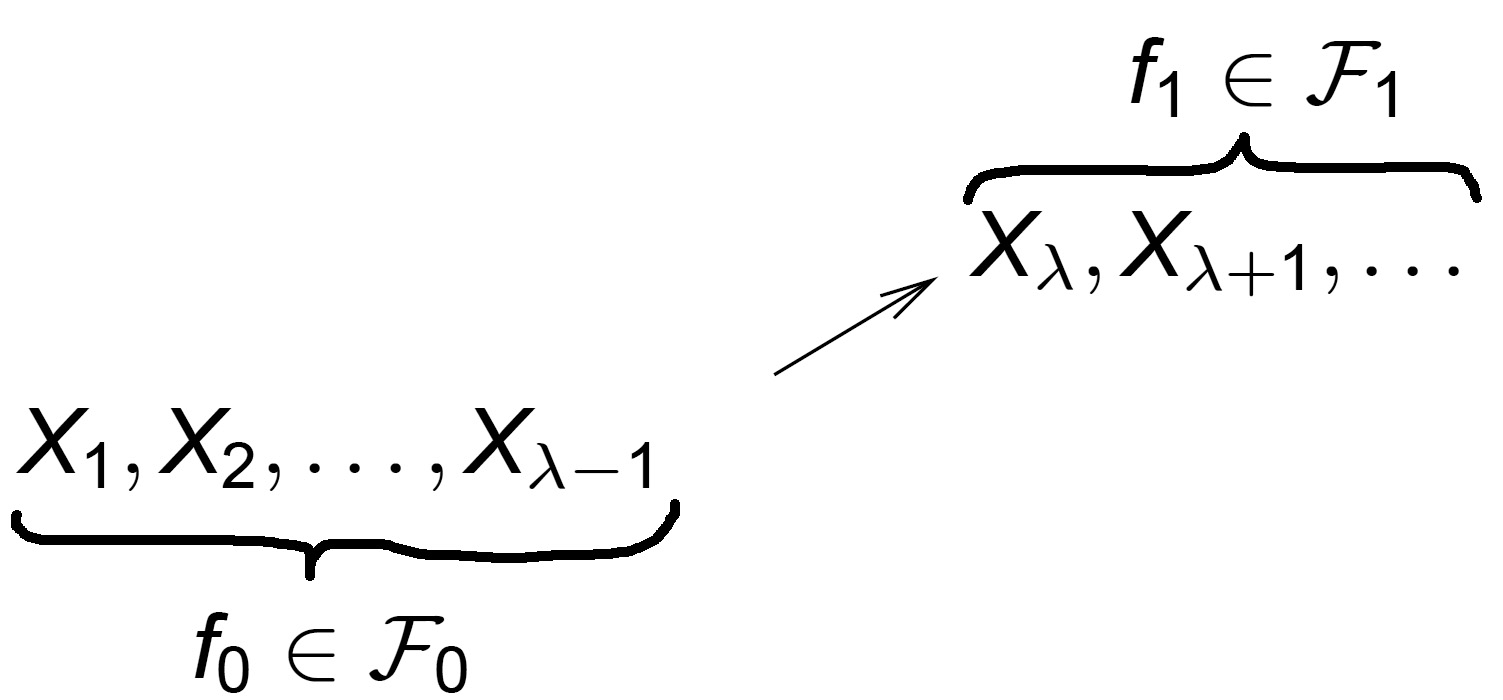
\includegraphics[width=0.5\linewidth]{PLOTS/generalized_likelihood_ratio.jpg} \hfill \mbox{ }}
\only<3>{\vspace{-3.3 cm} \hfill 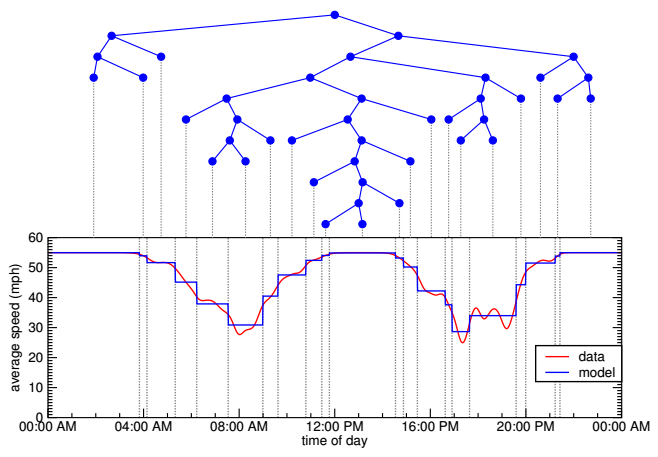
\includegraphics[width=0.6\linewidth]{PLOTS/tree_as_timesequence.png}}
\only<4>{\mbox{ } \hfill 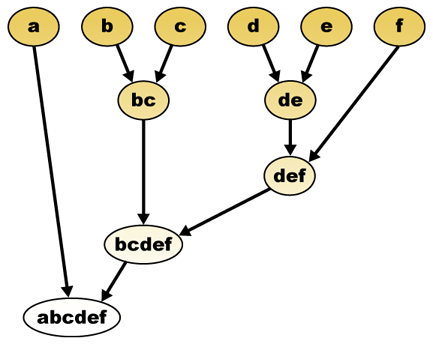
\includegraphics[width=0.4\linewidth]{PLOTS/hierarchical_diagram.png} \hfill \mbox{ }}
\end{frame}

\begin{frame}
\frametitle{Potential applications in physics}

\vspace{0.5 cm}
\begin{columns}
\column{0.5\linewidth}
Some quantities, such as the CMS magnetic field, have been simulated in high detail, but a simplified model must be used in tracking because of memory constraints.

\column{0.5\linewidth}
One could again use a regression tree, this time with $r$, $\phi$, $z$ as regressors, rather than time, to split the space by importance.

\mbox{ }
\end{columns}

\vspace{0.2 cm}
\begin{columns}
\column{0.7\linewidth}
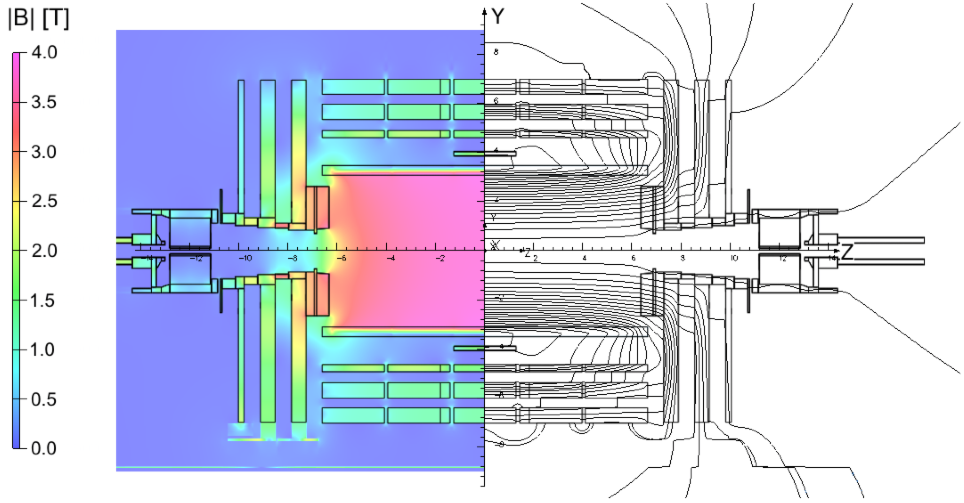
\includegraphics[width=\linewidth]{PLOTS/Sections_IntroductionFigs_MagField.png}

\column{0.3\linewidth}
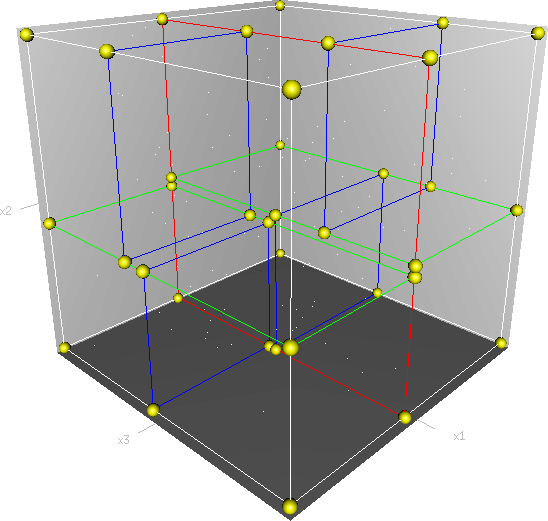
\includegraphics[width=\linewidth]{PLOTS/3dtree.png}
\end{columns}

\vspace{0.5 cm}
This is an example of using a model as compression (not even ``data'').
\end{frame}

\begin{frame}
\frametitle{Potential applications in physics}

\begin{columns}
\column{0.8\linewidth}
Physics is not the only field in which data quality must be monitored by human operators.

\vspace{0.1 cm}
Projects with large numbers of distributions to watch use anomaly detection models as the first pass.
\column{0.2\linewidth}
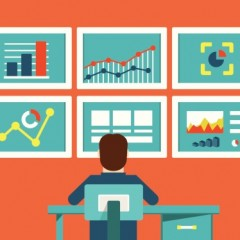
\includegraphics[width=\linewidth]{PLOTS/data_quality_monitoring.jpg}
\end{columns}

\begin{itemize}
\item CUSUM (cumulative sum) models catch slowly drifting trends, in which the accumulation of recent past is more significant than any one outlier.

\item Holt-Winters is an extension \\ of Exponentially Weighted \\ Moving Average (EWMA) \\ that can absorb complex \\ behaviors, such as cycles, \\ into the ``normal'' \\ distribution.
\end{itemize}

\vspace{-3.2 cm}
\hfill 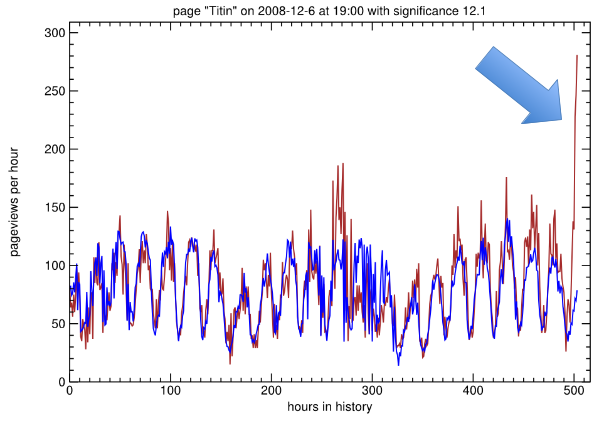
\includegraphics[width=0.5\linewidth]{PLOTS/holt-winters.png}
\end{frame}

\begin{frame}
\frametitle{Potential applications in physics}

\vspace{0.2 cm}
Non-linear regression is probably HEP's favorite \\ model, but in some cases, one does not want to \\ assume an ansatz (e.g.\ background combinatorics).

\vspace{-1.3 cm}
\hfill 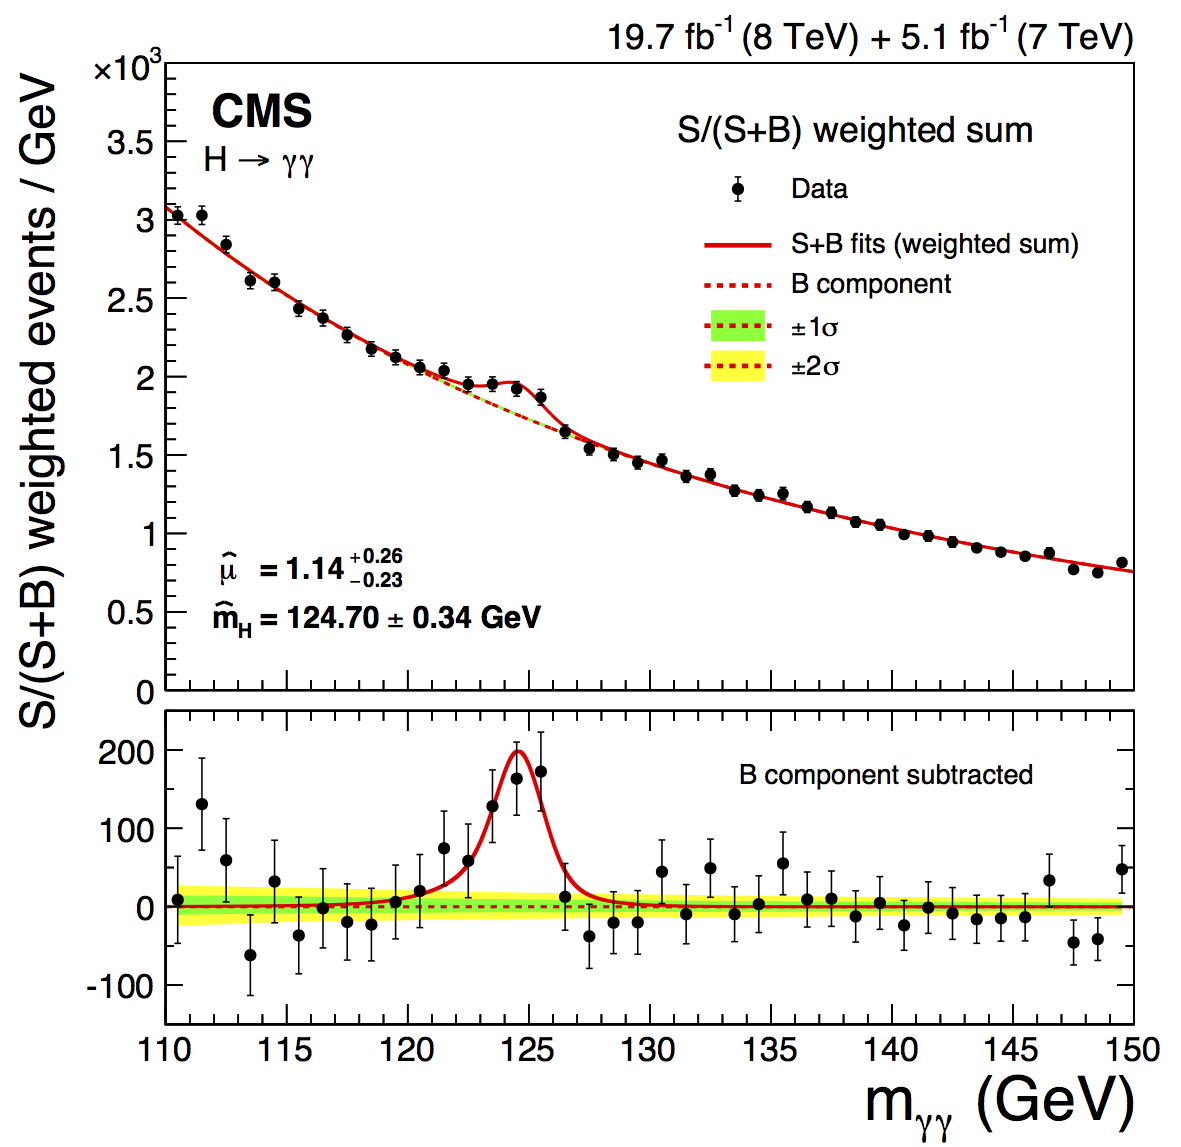
\includegraphics[width=0.28\linewidth]{PLOTS/higgs_gamma_gamma.png}

\vspace{-1.3 cm}
\textcolor{darkblue}{Non-parametric fitting techniques:}

\begin{itemize}

\item K-Nearest Neighbors (KNN): make a curve by \\ averaging the $k$ nearest points from the training dataset. \\ Alternatively, average all points within a ball of specified radius.

\item Locally Weighted Scatterplot Smoothing \\ (LOWESS): make a curve by linearly fitting \\ the training dataset $\{x_i\}$ at each $x_p$ with \\ weight $w_i = e^{-(x_i - x_p)^2/2/\sigma}$.

\vspace{-2.1 cm}
\hfill 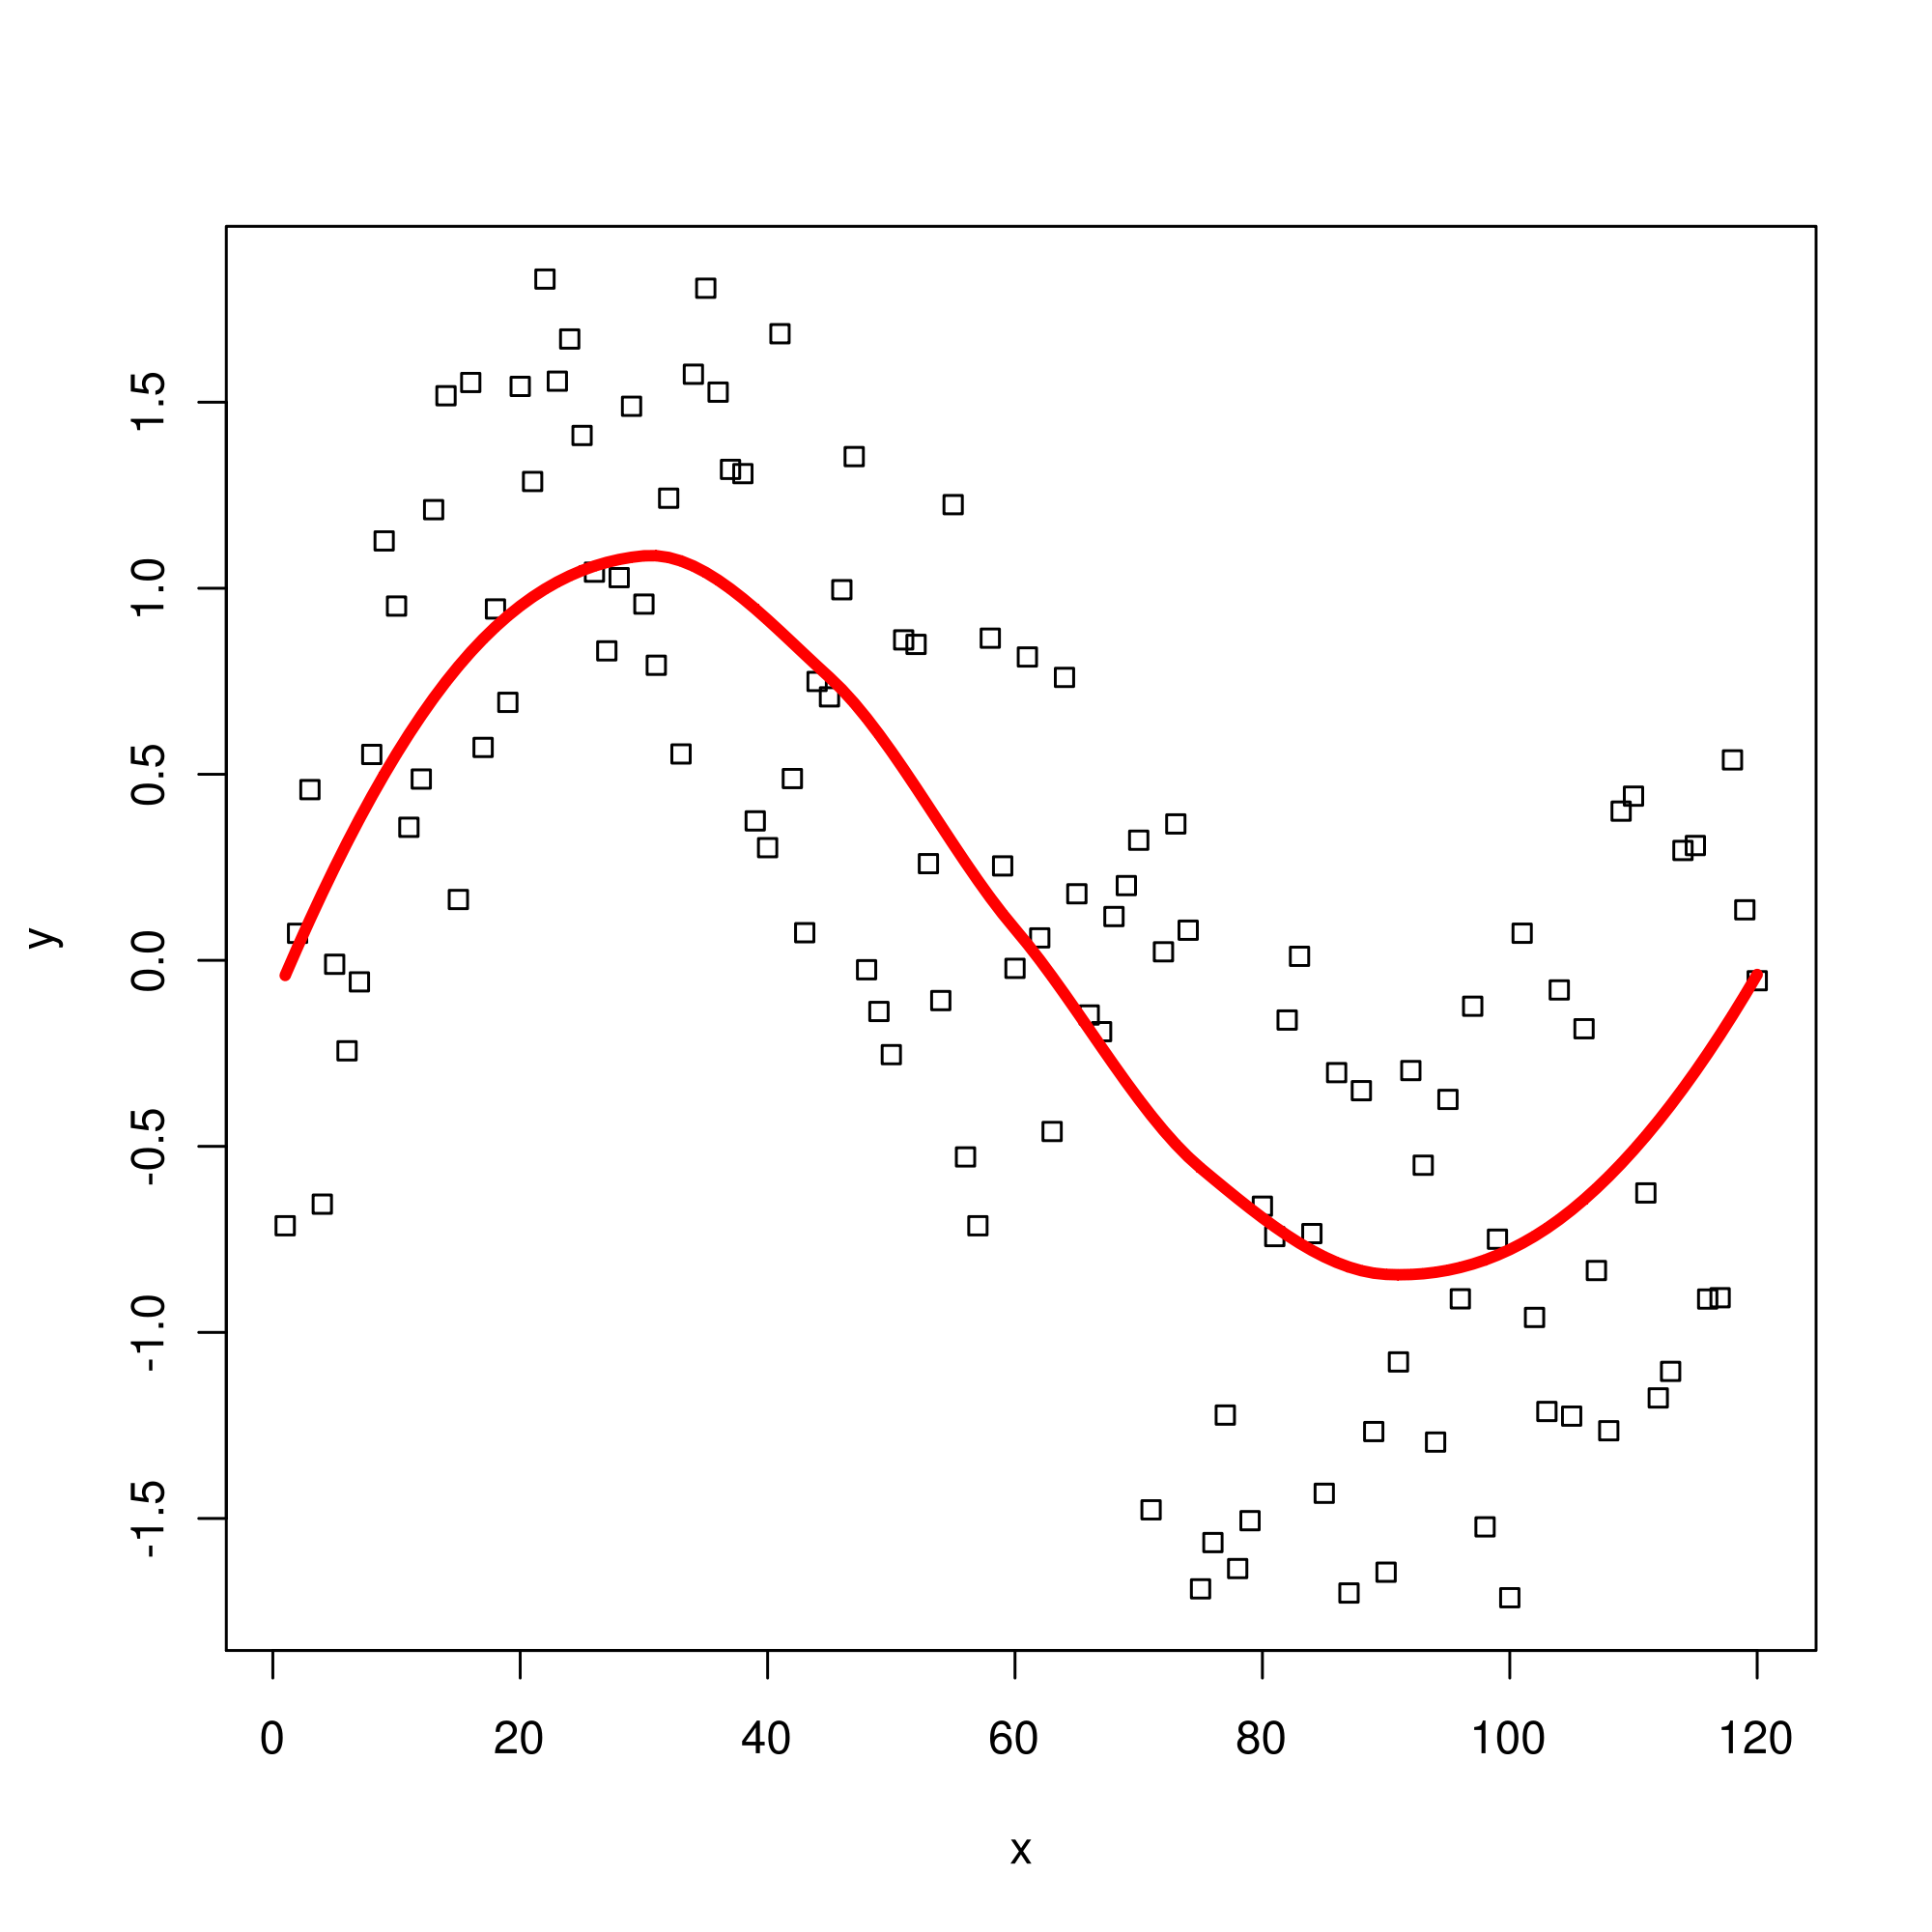
\includegraphics[width=0.3\linewidth]{PLOTS/loess.png}

\vspace{-0.4 cm}
\item Gaussian Process: make a curve by assuming nearby points to be more correlated than distant points.
\end{itemize}
\end{frame}

\begin{frame}
\frametitle{Spectrum of regression}
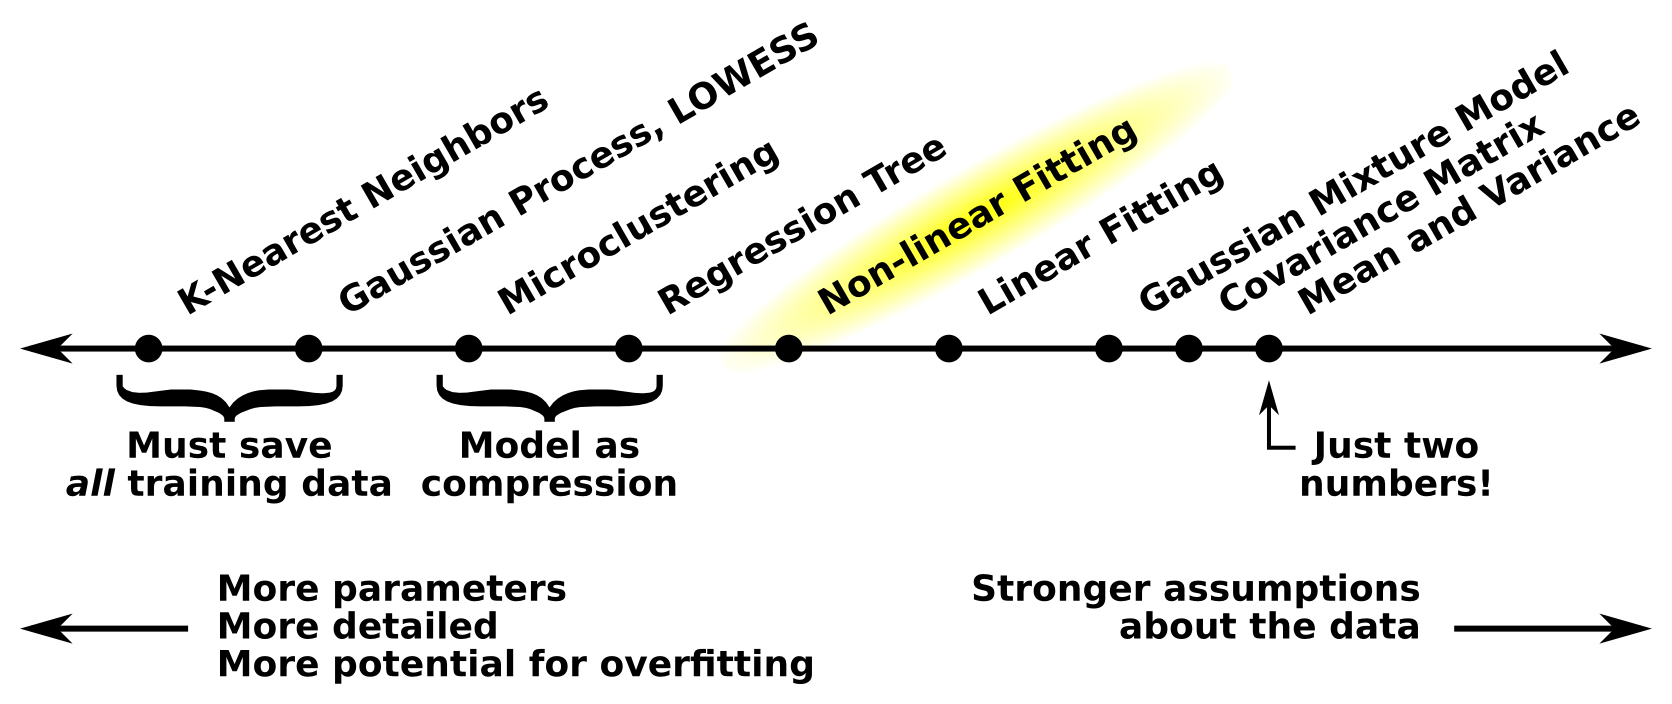
\includegraphics[width=\linewidth]{PLOTS/spectrum_of_regression.png}
\end{frame}

\section*{Software tools}
\begin{frame}
\begin{center}
\Huge \textcolor{blue}{Software tools}
\end{center}
\end{frame}

\begin{frame}
\frametitle{Big Data}

For decades, HEP had the biggest datasets anywhere.

\vfill
In the past 10--15 years, internet-related datasets have reached TB and PB scales: advertisement click-throughs, shopping correlations, web search engines, cybersecurity, Facebook pictures, YouTube videos, etc.

\vfill
\uncover<2->{But analyses of these datasets are also {\it tightly coupled.} For example,
\begin{itemize}
\item A customer buys diapers online; what other products should you recommend?
\item Analysis of diaper purchases across all customers reveals a correlation with milk; recommend milk.
\end{itemize}
The dataset, originally indexed by customer, must be re-indexed by product (or even by sets of products) to make a recommendation.}

\vfill
\uncover<3->{By contrast, most HEP analyses can process events independently.}
\end{frame}

\begin{frame}
\frametitle{Big Data}

\begin{description}
\item[Big Data (my definition):] a dataset that is too large to be processed on one computer; must resort to a distributed calculation.
\end{description}

\vspace{0.2 cm}
Distributed calculations are qualitatively different from in-memory calculations.

\vspace{0.2 cm}
They get increasingly difficult as the problems get more tightly coupled, since data must be shuffled among processors.

\begin{center}
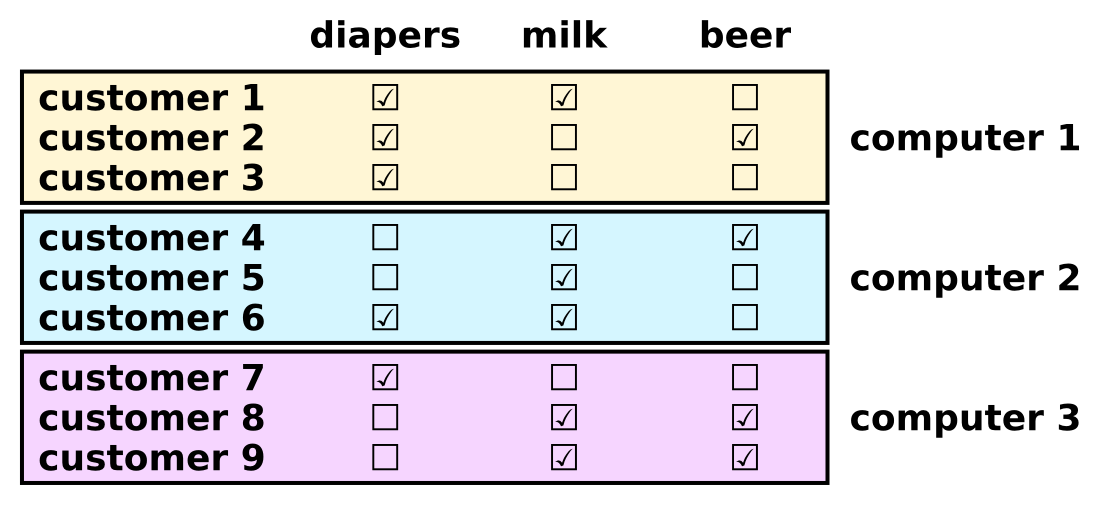
\includegraphics[width=0.8\linewidth]{PLOTS/distributed_data.png}
\end{center}
\end{frame}

\begin{frame}
\frametitle{Big Data}

Google had an re-indexing problem: a set of webpages containing words had to be re-indexed as a set of words pointing to webpages, so that you can search for pages by keyword.

\vfill
\uncover<2>{\begin{columns}
\column{0.41\linewidth}
Their solution, called ``map-reduce,'' was published as a white paper in 2004.

\vspace{0.2 cm}
It was immediately reimplemented as an open source product, \mbox{Apache Hadoop.\hspace{-1 cm}}

\column{0.25\linewidth}
\hfill 
\includegraphics[width=\linewidth]{PLOTS/01_Hadoop_full.jpg}

\column{0.15\linewidth}
\hfill 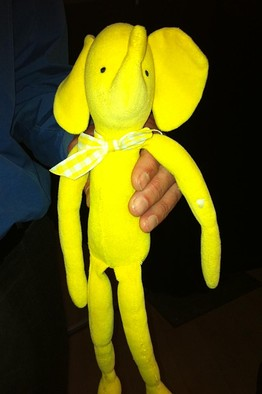
\includegraphics[width=\linewidth]{PLOTS/0605_cio_hadoop2_DV_20120605202616.jpg}
\end{columns}}

\vfill
\uncover<2>{Hadoop is now almost synonymous with Big Data, and it has spawned an ecosystem of tools that interoperate with it, much like ROOT in HEP.}
\end{frame}

\begin{frame}[fragile]
\frametitle{Map-reduce}

Hadoop executes two sets of independent, identical processors:
\begin{itemize}
\item Mappers, which transform each input to a $\langle$key, value$\rangle$ pair.
\item Reducers, each operates on all values that have a given key.
\end{itemize}

\vspace{-0.1 cm}
\begin{columns}
\column{0.5\linewidth}
\begin{lstlisting}[frame=single]
def mapper($webpage$):
  for $word$ in $webpage$.split():
    yield ($word$, $webpage$)
$$
\end{lstlisting}
\column{0.58\linewidth}
\begin{lstlisting}[frame=single]
def reducer($word$, $webpages$):
  searchIndex[$word$] = {}
  for $webpage$ in $webpages$:
    searchIndex[$word$].add($webpage$)
\end{lstlisting}
\end{columns}

The system groups data by key in an optimized way (independent partial sorts followed by merge, minimizing network bandwidth).

\vspace{0.2 cm}
\mbox{ } \hfill 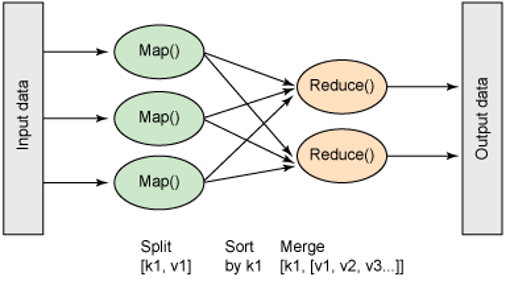
\includegraphics[width=0.6\linewidth]{PLOTS/mapreduce-diagram-by-ibm.png} \hfill \mbox{ }
\end{frame}

\begin{frame}[fragile]
\frametitle{Potential application in physics}

Most physics analyses apply the same function to all \mbox{events independently.\hspace{-1 cm}}

However, alignment and calibration are more tightly coupled:
\begin{itemize}
\item Alignment residuals must be re-indexed from tracks to subdetectors.
\item Calibration responses must be re-indexed from $\pi^0$s to subdetectors.
\end{itemize}

\begin{lstlisting}[frame=single]
def mapper($event$):
    for $track$ in $event$:
        for $hit$ in $track$:
            key = $hit$.subdetector()
            residual = $track$.projection($hit$) - $hit$.pos()
            yield (key, residual)
\end{lstlisting}

\begin{lstlisting}[frame=single]
def reducer($subdetector$, $residuals$):
    numer = 0
    denom = 0
    for $residual$ in $residuals$:
        numer = numer + $residual$
        denom = denom + 1
    >move>($subdetector$, numer/denom)  # shift by residual mean
\end{lstlisting}

Map-reduce can be applied to {\it one iteration} of alignment or calibration.
\end{frame}

\begin{frame}
\frametitle{Iterative map-reduce}

Hadoop was not designed for iterative map-reduce.

\vspace{0.5 cm}

\begin{columns}
\column{0.2\linewidth}

\includegraphics[width=\linewidth]{PLOTS/spark-logo.png}
\column{0.7\linewidth}

\vspace{0.2 cm}
Apache Spark is a framework that runs within a Hadoop cluster to speed up iteration.
\end{columns}

\vfill
\begin{columns}
\column{0.5\linewidth}
It provides more control over the workflow topology (not just {\tt map} and {\tt reduce}) and allows the user to cache some datasets in RAM memory, so that they don't have to be re-loaded from disk.
\column{0.4\linewidth}
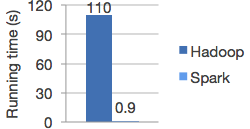
\includegraphics[width=\linewidth]{PLOTS/spark_time.png}
\end{columns}

\vspace{0.5 cm}
Disk access is the biggest bottleneck for calculations of this type.
\end{frame}

\begin{frame}[fragile]
\frametitle{Alignment example in Spark}

\begin{lstlisting}
@case class Ratio(numer, denom):
    def add(self, other):
        return >Ratio>(self.numer + other.numer,
                     self.denom + other.denom)
    def value(self):
        return self.numer / self.denom

def makePair($track$, $hit$):
    key = $hit$.subdetector()
    residual = $track$.projection($hit$) - $hit$.pos()
    return (key, >Ratio>(residual, 1))
\end{lstlisting}

\begin{lstlisting}[frame=single]
$tracks$.cache()   # tells Spark to keep tracks in memory

for $iteration$ in range(100):
    keyValuePairs =
        $tracks$.flatMap(lambda $track$: $track$.hits.map(
                         lambda $hit$: >makePair>($track$, $hit$)))

    corrections =
        keyValuePairs.reduceByKey(lambda r1, r2: r1.>add>(r2))
                     .mapValues(lambda r: r.>value>())

    corrections.foreach(>move>)
\end{lstlisting}
\end{frame}

\begin{frame}
\frametitle{Streaming calculations}

Another common problem in industry: how to perform distributed calculations in real-time?
\begin{itemize}
\item Example: update shopping correlations while customers are shopping, so that recommendations are based on purchases made in the last few minutes.
\end{itemize}

\vspace{0.2 cm}
Hadoop and Spark are batch processors: they work on one big dataset.

\vspace{0.2 cm}
\uncover<2>{Storm (and others, including ``Spark-Streaming'') are streaming processors: data flow through continuously.}

\vspace{0.2 cm}
\uncover<2>{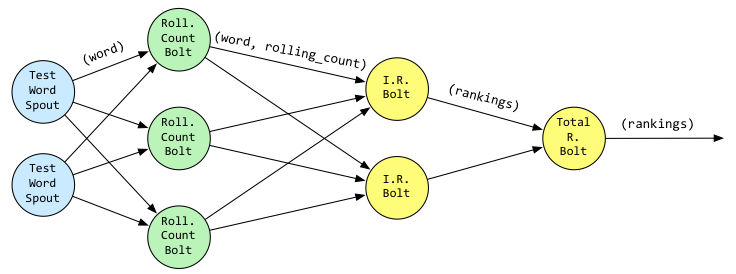
\includegraphics[width=0.8\linewidth]{PLOTS/Storm_rolling-count_topology.png}}

\vspace{-3.0 cm}
\uncover<2>{\hfill \begin{minipage}{0.46\linewidth}
\raggedleft
Processors pass events through a directed, acyclic graph.

\vspace{1.2 cm}
Fail-fast: if a processor encounters an error, it is immediately killed and replaced.
\end{minipage}}
\end{frame}

\begin{frame}
\frametitle{Streaming calculations}

Streaming processors can die and drop events, or the wrong version of code might be deployed online, so they are less trustworthy than the $N^{\mbox{\scriptsize th}}$ revision of a batch calculation.

\vspace{0.2 cm}
However, batch calculations are not up-to-date. Want best of both\ldots

\uncover<2>{\vspace{0.5 cm}
\hspace{-0.83 cm} \textcolor{darkblue}{\Large Lambda architecture}

\vspace{0.2 cm}
Solution: run both. Batch-process everything up to the last hour, stream-process starts fresh each hour, and queries combine results.

\vspace{0.2 cm}
\mbox{ } \hfill 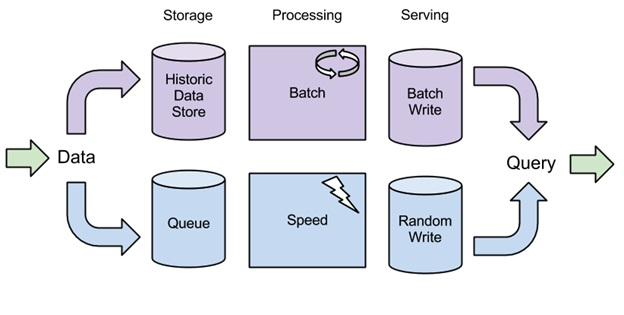
\includegraphics[width=0.8\linewidth]{PLOTS/Lambda-architecture-illustration.jpg} \hfill \mbox{ }}
\end{frame}

\section*{Programming trends}
\begin{frame}
\begin{center}
\Huge \textcolor{blue}{Programming trends}
\end{center}
\end{frame}

\begin{frame}
\frametitle{Language choice}

Everything mentioned so far was written in Java (or Scala or Clojure) with hooks for Python and R. Little support for C/C++. Why is that?

\vfill
\uncover<2->{\renewcommand{\arraystretch}{1.0} \begin{tabular}{>{\raggedright}p{0.3\linewidth} >{\raggedright}p{0.3\linewidth} >{\raggedright\arraybackslash}p{0.3\linewidth}}
\textcolor{darkblue}{C/C++} & \textcolor{darkblue}{JVM (Java et al)} & \textcolor{darkblue}{Python and R} \\
\vspace{-0.2 cm} Hardest to debug. Mixes analysis with low-level concerns. & \vspace{-0.2 cm} Human-readable internals, stack traces, runtime types. & \vspace{-0.2 cm} Interactive prompt! Everything can be inspected at runtime. \\
\uncover<3->{Fastest, raw machine access, \mbox{static bytecode,\hspace{-1 cm}} manual memory management.} & \uncover<3->{Medium speed, dynamic optimizer.} \only<3-4>{Garbage collector is fast but pauses.} \only<5>{\fbox{\begin{minipage}{\linewidth} \raggedright Garbage collector is fast but pauses. \end{minipage}}} & \uncover<3->{Slowest, though performance-critical code is external.} \\
\uncover<4->{Used by physicists (and cybersecurity).} & \uncover<4->{Used for large-scale business analytics; suited to networking.} & \uncover<4->{Used by statisticians and data scientists for laptop-analyses.}
\end{tabular}}
\end{frame}

\begin{frame}
\frametitle{Garbage collectors are actually fast}

Static memory management fragments the heap, so the ``new'' (or ``malloc'') command has to {\it search} for an available block.

\mbox{ } \hfill 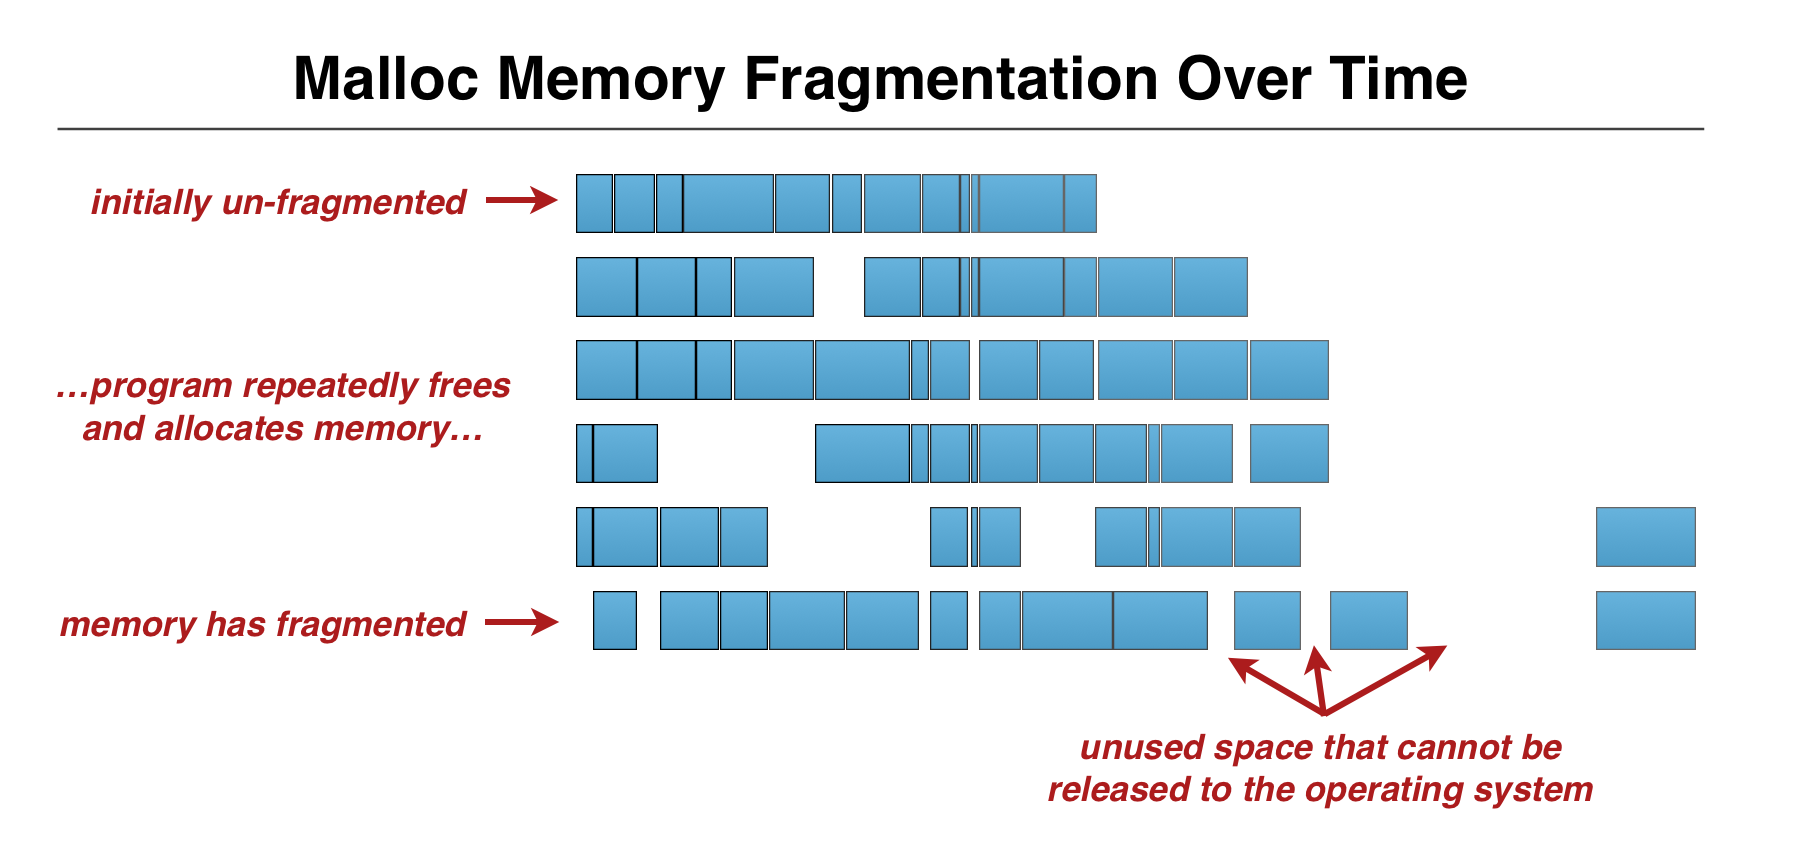
\includegraphics[width=0.7\linewidth]{PLOTS/malloc_memory_fragmentation.png} \hfill \mbox{ }

Managed memory fills like a stack, so there is no search, and the whole stack is cleared when surviving objects are moved to longer-term storage.

\mbox{ } \hfill 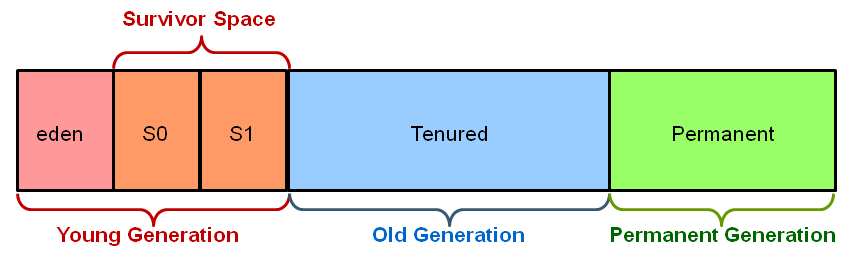
\includegraphics[width=0.7\linewidth]{PLOTS/jvm_gc.png} \hfill \mbox{ }
\end{frame}

\begin{frame}
\frametitle{Garbage collectors are actually fast}

New/delete (malloc/free) memory management:

\begin{center}\renewcommand{\arraystretch}{1.5}
\begin{tabular}{| c | c | c |}
\hline new & delete & random pauses \\\hline
slow & fast & don't happen \\\hline
\end{tabular}
\end{center}

Garbage collectors:

\begin{center}\renewcommand{\arraystretch}{1.5}
\begin{tabular}{| c | c | c |}
\hline new & delete & random pauses \\\hline
fast & n/a & happen \\\hline
\end{tabular}
\end{center}

\uncover<2>{\begin{itemize}
\item Good for most distributed applications because network data is intermittent; pauses fill the cracks.
\item Worked against a high-throughput application I wrote: input stream was continuous, so garbage collector pauses caused data to overflow the input queue. {\it Would have been better slower and uniform!}
\end{itemize}}
\end{frame}

\begin{frame}[fragile]
\frametitle{Immutable data}

Another trend is the restriction to immutable data: variables that don't vary and data structures that can only be replaced, not changed.

\vspace{0.5 cm}
\begin{columns}
\column{0.4\linewidth}
Mutable variable:

\begin{lstlisting}[frame=single]
result = 0
for i in range(10):
  result = result + i
>>
>>
>>
\end{lstlisting}

\vspace{0.3 cm}
Mutable data structure:

\begin{lstlisting}[frame=single]
result = []
for i in range(10):
  result.>append>(i)
>>
>>
>>
\end{lstlisting}

\column{0.5\linewidth}
Immutable variable:

\begin{lstlisting}[frame=single]
def add(i):
  if i < 10:
    return i + >add>(i+1)
  else:
    return 0
result = >add>(0)
\end{lstlisting}

\vspace{0.3 cm}
Immutable data structure:

\begin{lstlisting}[frame=single]
def appended(i):
  if i < 10:
    return [i] + >appended>(i+1)
  else:
    return []
result = >appended>(0)
\end{lstlisting}
\end{columns}
\end{frame}

\begin{frame}[fragile]
\frametitle{Immutable data}

Why impose this limitation? Because calculations are distributed.

\begin{itemize}
\item It is extremely difficult to maintain consistent values for mutable variables across computers in a network (CAP theorem).
\item Multiple threads in the same computer acting on a shared variable can easily corrupt it.
\end{itemize}

\vspace{0.75 cm}
Example: concurrent access to a mutable counter.

\begin{lstlisting}
def updateCounter():
    # step 1
    currentValue = getCounterValue()
    # step 2
    newValue = currentValue + 1
    # step 3
    setCounterValue(newValue)
\end{lstlisting}

\vspace{-4.5 cm}
\hfill 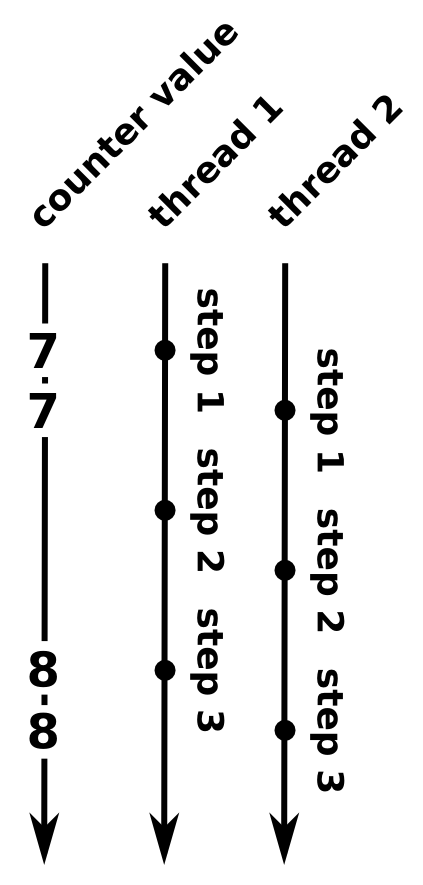
\includegraphics[width=0.23\linewidth]{PLOTS/time_mutable.png}
\end{frame}

\begin{frame}
\frametitle{Immutable data}

\begin{description}
\item[Curse of immutable data:] large data structures must be replaced by a new version for each change, suggesting an expensive copy.
\item<2->[Blessing of immutable data:] if immutable (and acyclic), multiple versions can share parts without {\it fully} copying.
\end{description}

\begin{columns}
\column{0.5\linewidth}
\uncover<2->{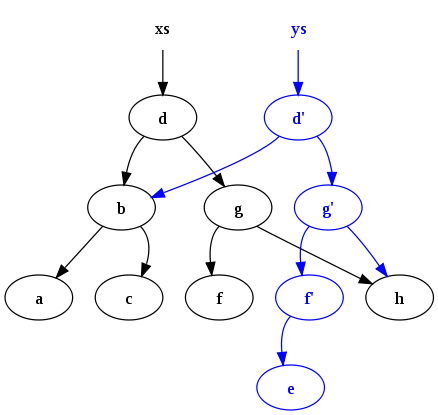
\includegraphics[width=\linewidth]{PLOTS/438px-Purely_functional_tree_after.png}}
\column{0.5\linewidth}
\uncover<2->{{\tt \textcolor{blue}{ys} = xs with \textcolor{blue}{e} added to f}

\vspace{0.2 cm}
Only the path from {\tt f} to root needs to be duplicated.}

\vspace{1 cm}
\renewcommand{\arraystretch}{1.5}
\uncover<3>{\begin{tabular}{c | c c}
& update & ``copy'' \\\hline
mutable & $\mathcal{O}(1)$ & $\mathcal{O}(n)$ \\
immutable & $\mathcal{O}(\log(n))$ & $\mathcal{O}(1)$
\end{tabular}}
\end{columns}
\end{frame}

\begin{frame}[fragile]
\frametitle{Monoids for combining results}

A monoid is a group without inverses:
\begin{itemize}
\item an identity: $0$ for which $a + 0 = a$
\item an associative operator: $a + (b + c) = (a + b) + c$
\end{itemize}

\vspace{0.2 cm}
\mbox{ } \hfill 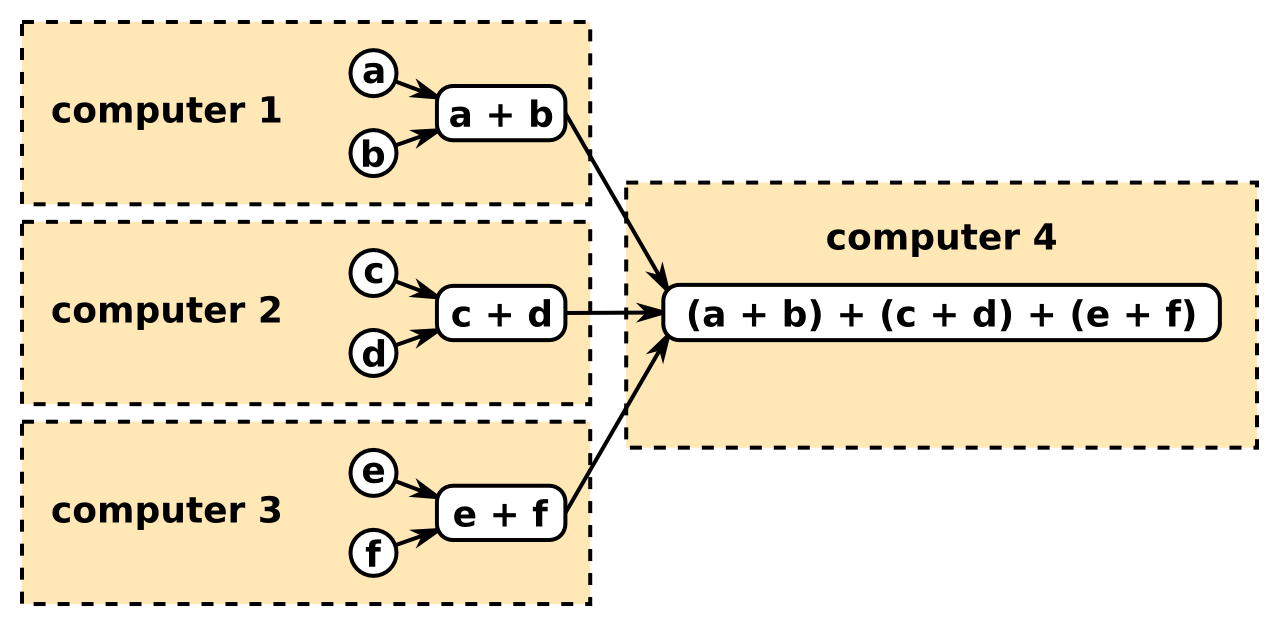
\includegraphics[width=0.7\linewidth]{PLOTS/monoids.png} \hfill \mbox{ }

\vspace{0.2 cm}
\begin{lstlisting}
@case class Ratio(numer, denom):
    def add(self, other):
        return >Ratio>(self.numer + other.numer,
                     self.denom + other.denom)
    def value(self):
        return self.numer / self.denom
\end{lstlisting}
\end{frame}

\begin{frame}
\frametitle{Actors for encapsulating work}

A distributed calculation can be made out of small, single-threaded mini-programs called Actors.

\vspace{0.2 cm}
\begin{itemize}
\item Actors have a mailbox that accumulates messages in a queue.
\item Their only behavior is to react to these messages, one at a time.
\item They can send messages to other actors.
\item They can freely use \\ mutable variables to \\ process a message, and \\ may or may not be \\ allowed to maintain \\ persistent, mutable state. \\ (Would not be fail-fast.)
\item The Akka framework is a \\ popular example.
\end{itemize}

\vspace{-3.8 cm}
\hfill 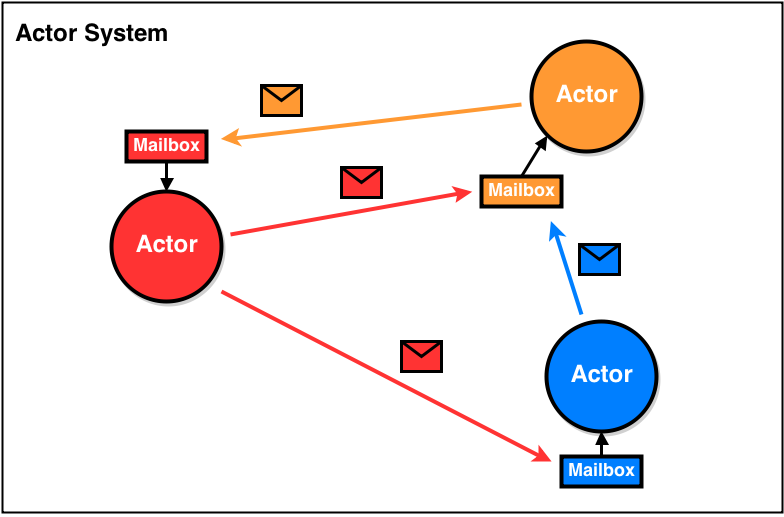
\includegraphics[width=0.55\linewidth]{PLOTS/ActorModel.png}
\end{frame}

\begin{frame}
\frametitle{Last topic: static typing}

C/C++ and Java declare and check data types during compilation to generate more efficient bytecode.

\vspace{0.2 cm}
Python and R only check types immediately before they are used.

\vspace{0.2 cm}
But a compile-time (static) type check is also a great way to prevent human error, especially in large or long-running calculations.
\uncover<2>{\begin{itemize}
\item My most common bug involved a Python {\tt None} (representing a missing value) entering arithmetic expressions.
\item Requiring explicitly named classes is safer than generic tuples or argument lists with many parameters of the same type.
\item Wrappers around numbers prevents unit mismatches, as does CMSSW's distinction between vectors and affine points.
\item A type check for matrix dimensions would be a great tool.
\end{itemize}}
\end{frame}

\begin{frame}[fragile]
\frametitle{Last topic: static typing}

Example: preventing all ``null'' errors at runtime.
\begin{itemize}
\item C/C++ raises a segmentation fault when reading {\tt NULL} pointers.
\item Java raises an exception that provides a line number in the code.
\item Python's null is {\tt None}, which raises an exception if you try to use it in arithmetic.
\item Some languages convert it to zero and move on!
\end{itemize}

\vfill
Scala has a wrapper type for objects that could be null: {\tt Option[T]}.

\begin{lstlisting}[language=java]
var x: Option[Double] = Some(3.14)
x = None

var y: Double = x match {
  case Some(y) => y + 3     // y is a new variable
  case None => -999         // no new variables in this scope
}
\end{lstlisting}

The type system forces the programmer to handle the null case; the above code will never raise an exception at runtime.
\end{frame}

\begin{frame}
\frametitle{Conclusions}

\begin{itemize}
\item Data scientists cover the same range of activities as experimental high-energy physicists, but work with a broader class of models for more diverse purposes.

\item Some of these statistical techniques could be useful in physics.

\item The software tools could be useful as well:
\begin{itemize}
\item Spark for iterative map-reduce could formalize and accelerate alignment and calibration.
\item Streaming processors or a lambda architecture could aid data monitoring.
\end{itemize}

\item Data scientists use more high-level programming languages and techniques, which reduce debugging time.
\begin{itemize}
\item Doesn't have to be the JVM. New languages (Rust, Julia, Numba just-in-time compiler for Python) produce native bytecode with high-level abstractions.
\end{itemize}
\end{itemize}

\label{numpages}
\end{frame}

\end{document}
